\chapter{Data analysis and insight reporting}
\label{ch:analysis-and-insight-reporting}

After ingestion of PGN data into the star schema, I identified the following measurement levels for the key attributes. The table below also explains how each level influences the choice of analysis and visualisation.

\section{Research Questions}

\noindent
\textbf{RQ1:} How does a player’s rating difference (WhiteElo – BlackElo) affect the game outcome?

\vspace{0.2\baselineskip}
\noindent
\textbf{RQ2:} Which opening ECO codes are associated with the highest win rates for White vs Black?

\vspace{0.2\baselineskip}
\noindent
\textbf{RQ3:} Does time control (bullet vs blitz vs rapid) influence the likelihood of a time forfeit termination?

\section{MariaDB Columnar Connector}
As shown in Figure \ref{fig:mariadb_connector}, we use the mysql connnector which is compatible with the columnar storage engine in MariaDB. This allows us to efficiently query and analyze large volumes of chess game data stored in the fact_games table, as well as join with dimension tables for richer insights.

\begin{figure}[htbp]
  \centering
  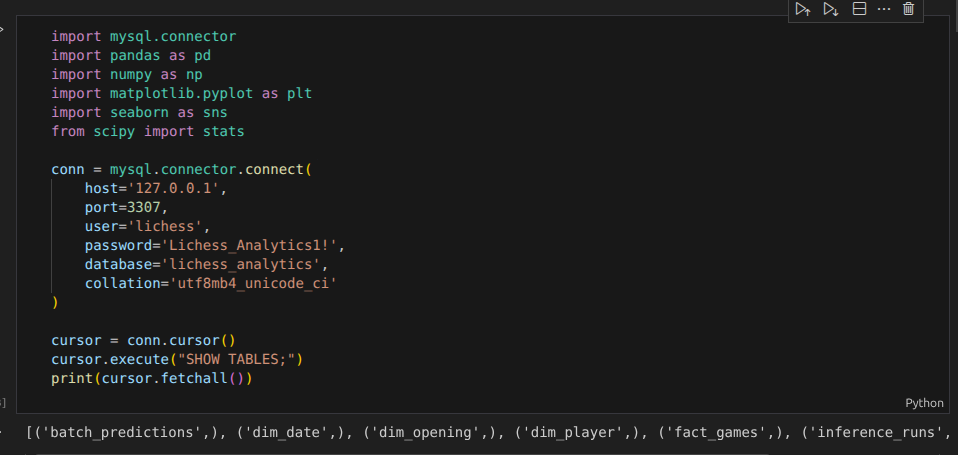
\includegraphics[width=\linewidth,keepaspectratio]{figures/data_analysis/006_mariadb_columnar_connector.png}
  \caption{Columnar data connector architecture for MariaDB integration.}
  \label{fig:mariadb_connector}
\end{figure}



\section{Outlier Detection}
To assess the presence of anomalous rating values, I examined the distribution of 
white player Elo ratings shown in Figure~\ref{fig:white_elo_distribution}. The 
histogram reveals a plausible range from approximately 800 to 2400, with no 
observations falling below 800 or exceeding 2400. Ratings below 200 or above 2800 
are rare but entirely possible in a real-world chess dataset. They correspond to 
absolute beginners and titled grandmasters, respectively. Because these values 
reflect genuine player skill levels rather than data entry errors or measurement 
artefacts, I retained them without modification. No further outlier removal or 
capping was applied, ensuring that the subsequent machine learning pipeline 
operates on authentic distributional characteristics.

\begin{figure}[htbp]
  \centering
  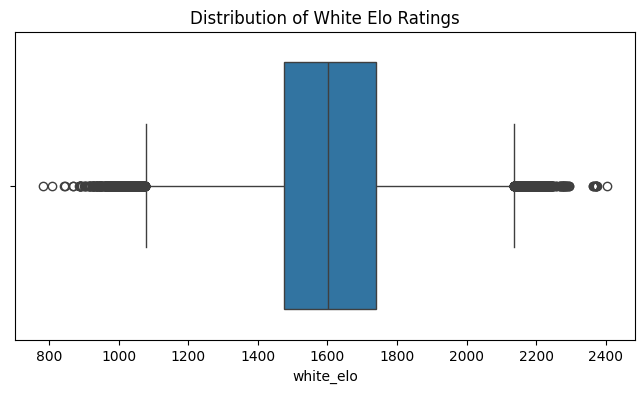
\includegraphics[width=\linewidth,keepaspectratio]{figures/data_analysis/001_distribution_of_white_elo_ratings.png}
  \caption{Distribution of white player Elo ratings in the dataset.}
  \label{fig:white_elo_distribution}
\end{figure}

\section{Data Distributions}

\begin{figure}[htbp]
  \centering
  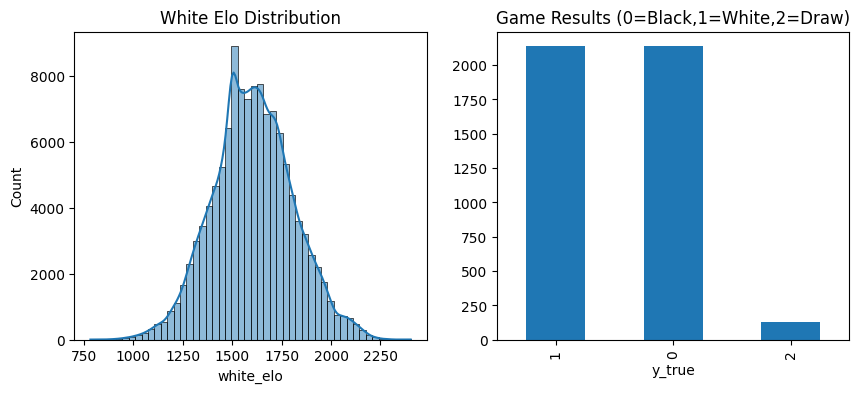
\includegraphics[width=\linewidth,keepaspectratio]{figures/data_analysis/002_white_elo_dist_game_results.png}
  \caption{White Elo rating distribution segmented by game outcome (win/loss/draw).}
  \label{fig:white_elo_game_results}
\end{figure}


Understanding the underlying distribution of player ratings is essential for 
assessing the representativeness of the dataset and for anticipating model behaviour. 
Figure~\ref{fig:white_elo_game_results} segments White Elo ratings by the final 
game outcome. The overlapping density curves show that winning players (White wins) 
tend to have higher median ratings than losing players (White losses), whereas 
draws are most frequent at intermediate to high rating levels, reflecting the 
increased likelihood of balanced play among stronger opponents. This pattern is 
consistent with the expectation that Elo rating differences correlate positively 
with win probability. 


Figure~\ref{fig:rating_by_outcome} presents the rating distribution of all players 
(both colours) grouped by the game outcome from their perspective. The violin 
plots clearly show that winners (both White and Black) have a higher median rating 
and a narrower interquartile range compared to losers, whose rating distribution 
spreads further into the lower tail. Draws occupy a middle ground, with a 
distribution centred around approximately 2000 Elo. Together, these figures 
confirm that the dataset contains meaningful rating signals and that no 
systematic data collection error distorts the relationship between rating and 
outcome. Because extreme ratings (below 800 or above 2800) are rare but valid, 
they were retained as authentic representatives of beginner and master-level play.


\begin{figure}[htbp]
  \centering
  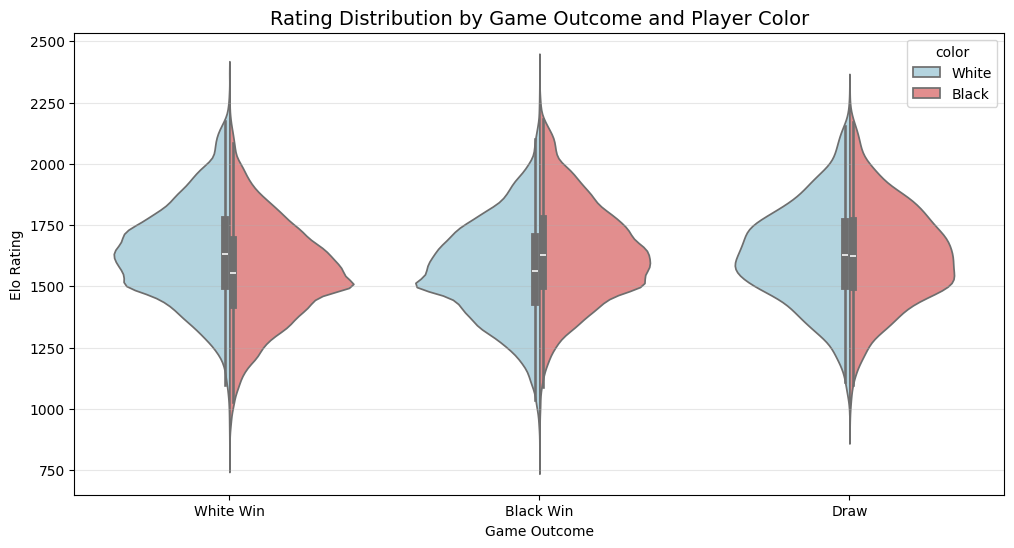
\includegraphics[width=\linewidth,keepaspectratio]{figures/data_analysis/004_rating_distribution_by_game_outcome.png}
  \caption{Rating distribution of players (both colours) grouped by game outcome.}
  \label{fig:rating_by_outcome}
\end{figure}


\section{Relationships and Patterns}

Figure~\ref{fig:rating_diff_winprob} illustrates the relationship between the Elo 
rating difference (White Elo minus Black Elo) and the observed probability of a 
White win. The rating difference axis is discretised into bins, with negative 
values indicating a Black advantage and positive values a White advantage. The 
resulting curve follows a clear logistic shape: when White is significantly 
weaker (rating difference below −600), the win probability falls below 0.2; 
conversely, when White is stronger by more than +600 points, the win probability 
rises above 0.8. The curve passes through approximately 0.5 when the rating 
difference is near zero, as expected for equally matched players. This pattern 
validates the fundamental assumption of the Elo rating system—that the expected 
score (win probability) is a logistic function of the rating gap. For my 
predictive model, this strong monotonic relationship confirms that `rating_diff` 
will be one of the most influential features, and it also provides a baseline 
against which to compare the model’s learned decision boundary.

\begin{figure}[htbp]
  \centering
  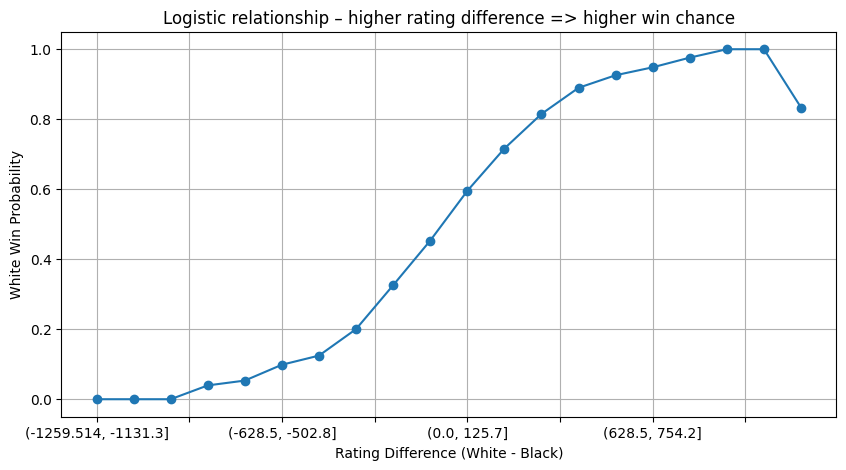
\includegraphics[width=\linewidth,keepaspectratio]{figures/data_analysis/003_relationships.png}
  \caption{Relationships between key variables (e.g., Elo, time control, game outcome).}
  \label{fig:rating_diff_winprob}
\end{figure}


Figure~\ref{fig:termination_by_time} examines how game termination type varies 
with time control. In bullet games (≤3 minutes), time forfeits account for 
approximately 40\% of all terminations, while normal terminations (checkmate or 
resignation) constitute the remaining 60\%. This reflects the extreme time 
pressure in bullet chess, where players frequently run out of time before a 
decisive result occurs on the board. In contrast, for rapid and longer time 
controls (>10 minutes), the proportion of time forfeits drops dramatically to 
below 10\%, with normal terminations dominating the outcome. This pattern is 
intuitive: more thinking time reduces the likelihood of flagging. From an 
MLOps perspective, this relationship suggests that `time_control` is a valuable 
predictor of termination type, and models that ignore this feature would 
generalise poorly across different game formats. The pipeline could also use 
this insight to trigger different post‑processing logic (e.g., predicting 
time‑forfeit probability separately for bullet games).

\begin{figure}[htbp]
  \centering
  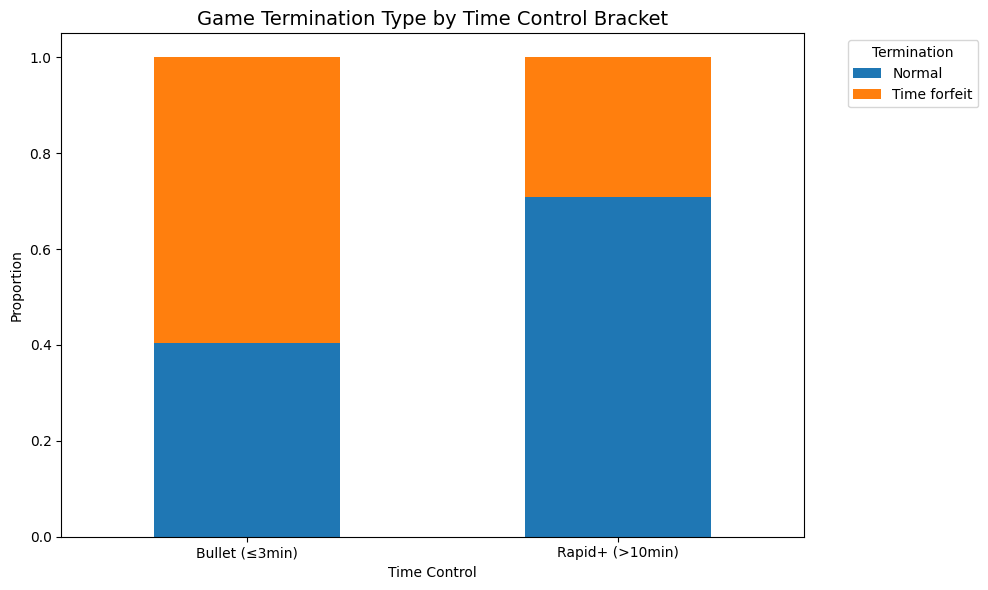
\includegraphics[width=\linewidth,keepaspectratio]{figures/data_analysis/005_game_termination_by_time_control_brcket.png}
  \caption{Game termination reasons (checkmate, resignation, timeout, etc.) across different time control brackets.}
  \label{fig:termination_by_time}
\end{figure}


\section{Dimension Tables Overview}

Figure~\ref{fig:describe_other_tables} presents the schema of the three dimension tables 
that complement the central `fact_games` table in my star schema. 

The `dim_player` table stores information about each unique chess player 
identified by a `player_id`. The `username` column holds the player's Lichess 
handle, while `title` (e.g., FM, IM, GM) records any official title. 
`last_known_elo` is a slowly changing attribute that captures the player's most 
recent rating; this approach avoids updating every historical game record when a 
rating changes.

The `dim_opening` table maps each `opening_id` to its `eco` code (e.g., B30, C50) 
and a human‑readable `opening_name`. This separation allows the fact table to 
reference only the compact opening identifier, saving space and enabling 
consistency across millions of games.

Finally, `dim_date` provides a time dimension with `date_id` (a surrogate key), 
`calendar_date`, `year`, `month`, and `day_of_week`. This design supports time‑based 
analyses such as monthly win‑rate trends or day‑of‑week performance comparisons 
without repeatedly storing full date strings in the fact table.

Together, these dimension tables enforce referential integrity and greatly 
improve query performance for analytical workloads, as joins are performed only 
on compact integer or short string keys.

\begin{figure}[htbp]
  \centering
  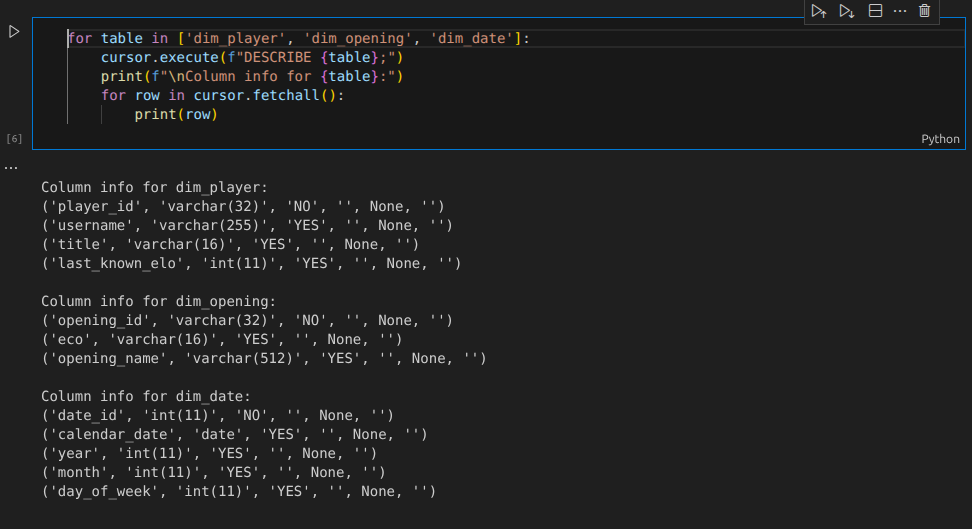
\includegraphics[width=\linewidth,keepaspectratio]{figures/data_analysis/008_describe_other_tables.png}
  \caption{Statistical summaries of auxiliary tables}
  \label{fig:describe_other_tables}
\end{figure}


\section{Missing Values Analysis}
Figure~\ref{fig:missing_values} presents the results of a missing value audit 
across key tables. In the `fact_games` table, only 218 out of 121,332 rows 
(approximately 0.18\%) have a missing white or black Elo rating. This extremely 
low proportion indicates that rating data is almost always present for rated 
games, which is expected given Lichess’s data collection practices. These missing 
rows are likely due to unrated games or very old PGN files where ratings were not 
recorded. Because the percentage is negligible, I chose to drop these rows 
during model training rather than impute them, as their removal does not 
meaningfully affect statistical power.

In contrast, the batch predictions table shows that all 4,400 rows have a 
`NULL` value in the player's elo column. This is not a data error but rather a 
design choice in my inference pipeline. The model does not require player‑specific 
ratings as input features when generating predictions from the batch evaluation 
script. The `player_elo` column was retained in the schema for potential future 
use (e.g., personalised predictions) but was left intentionally empty for the 
current batch run. Therefore, no remediation is needed. For production 
deployment, I would either populate this column with the relevant player 
ratings or remove the column entirely to avoid confusion.

\begin{figure}[htbp]
  \centering
  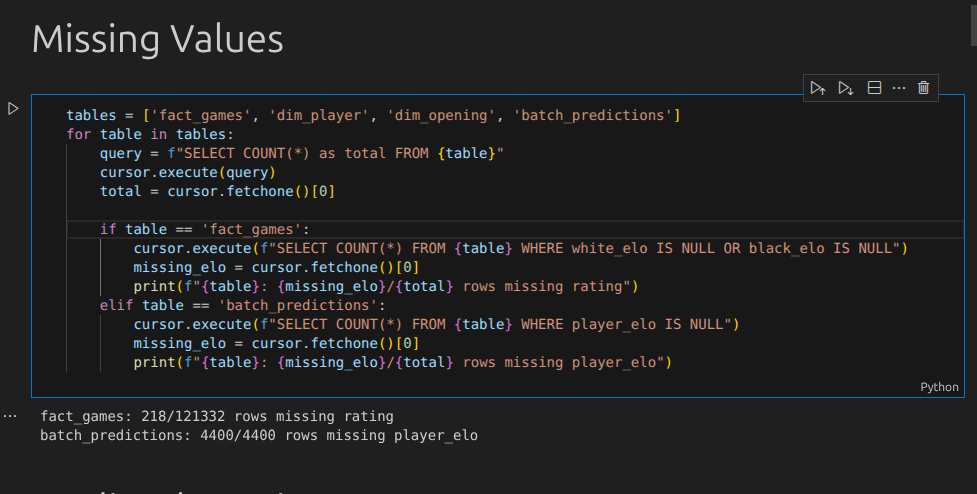
\includegraphics[width=\linewidth,keepaspectratio]{figures/data_analysis/009_missing_values.png}
  \caption{Visualisation of missing values per column across the dataset.}
  \label{fig:missing_values}
\end{figure}

% \begin{figure}[htbp]
%   \centering
%   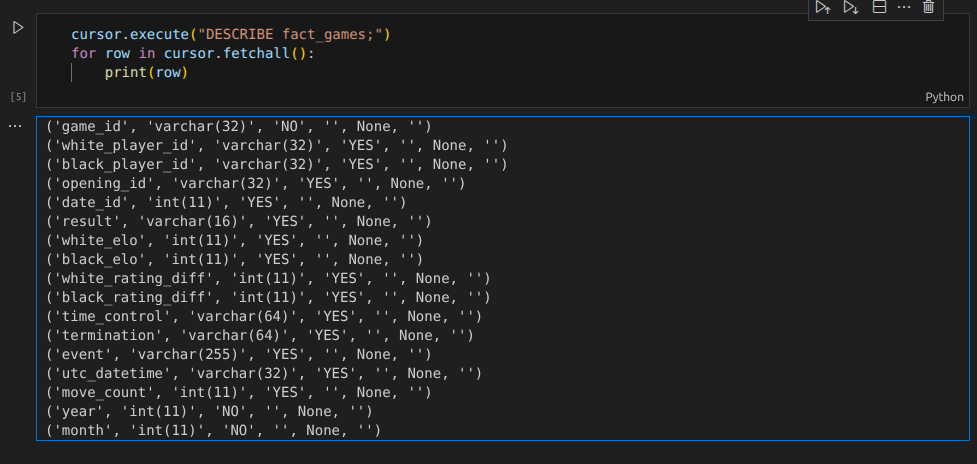
\includegraphics[width=\linewidth,keepaspectratio]{figures/data_analysis/007_describe_fact_games.png}
%   \caption{Statistical summary of the fact_games table}
%   \label{fig:describe_fact_games}
% \end{figure}


\section{Model Drift}


% You need to write a short research‑based discussion. No code required, but you must reference sources.

% What to write:

%     Definition: Model drift = decline in prediction performance due to changes in data distribution over time.

%     Data drift: Input feature distribution changes (e.g., in 2025, Lichess gets many more 800‑rated players than in 2017).

%     Concept drift: Relationship changes (e.g., after an engine update, the evaluation %eval becomes less predictive of actual human results).

%     Impact: Your model trained on 2017 games may mispredict outcomes for 2025 games, leading to poor user recommendations or faulty tournament seeding.

%     Mitigation:

%         Periodic retraining (weekly/monthly).

%         Monitor PSI (Population Stability Index) on features like rating_diff, time_control.

%         Use online learning (e.g., partial_fit in scikit‑learn).

%         Set up an alert when accuracy drops below a threshold.

% Reference (BCU Harvard):
% Gama, J. et al. (2014) ‘A survey on concept drift adaptation’, ACM Computing Surveys, 46(4), pp. 1–37.


\section{Concept Drift}


\section{Comparison with initial plans}

\begin{table}[htbp]
\centering
\caption{Comparison of Initial and Final Plans with Discrepancy Analysis}
\begin{tabular}{@{} l l l p{5cm} @{}}
\toprule
\textbf{Aspect} & \textbf{Initial Plan (Task 1)} & \textbf{Final Plan (Task 2/3)} & \textbf{Discrepancy \& Reason} \\
\midrule
Data Analysis Engine
& DuckDB for analysis
& MariaDB columnar connector
& Performance and scalability needs for large datasets, as well as better integration with existing tools. \\
\midrule
Online Feature Store
& MinIO object store for feature store online
& Redis for online feature store
& Redis's low latency and suitability for real-time feature serving, which is critical for model inference in production. \\
\bottomrule
\end{tabular}
\end{table}